\documentclass{article}
\usepackage{cite}
\usepackage{graphicx}
\usepackage{amsmath}
\newcommand\norm[1]{\left\lVert#1\right\rVert}
\DeclareMathOperator*{\argmin}{arg\,min}

\setlength{\parindent}{0cm}
\setlength{\parskip}{0.25cm}

\begin{document}
\author{Max Horowitz-Gelb}
\title{Active Learning For DBSI: DNA Binding Site Identifier }
\maketitle

\section*{Abstract}
DBSI is a structure based method for predicting the positions of protein interaction sites associated with DNA binding \cite{dbsi}. Here I present an application of active learning to DBSI based on the methods described in \cite{active_learning}. The method used optimizes the training of DBSI in a way that considers the batch style constraints of labelled data collection for DBSI. Evaluation of the method shows slight improvement over a naive method.
\section*{Introduction}
For area under an ROC curve, DBSI has been shown to achieve $~88\%$, a high degree of separability. The score was achieved by training DBSI on a set of 263 unique proteins. The model as a result of this training is now accessible to anyone on a public server \cite{dbsi_server}. The quality of this model could be improved further by training with more labelled data. But to do so requires practical considerations.
\subsection*{Necessity for Active Learning}
Unlike learning on data generated from sensors or internet activity, aquiring labelled data for DBSI requires considerable time and energy. Much of this labelled data can be generated computationally from protein-DNA complex databases as described in \cite{displar}.
But for many complexes, particularly for Protein-RNA complexes, much is still missing. To aquire data in these cases would require considerable lab work. Even for complexes that do exist in databases, there are thousands to choose from and one cannot reasonably extract all of them. 

These issues highlight the need for a method of finding data that best helps increase the quality of the predictive model. Active learning methods do just this. The goal of these methods is to iteratively request new training data with the hope of maximizing the quality increase with each new training instance added. When selecting training instances, also known as querying, the active learner only has knowledge of the input features, not the label. This is useful for DBSI since the features may be available for each protein, but aquiring a label come at some cost of time and effort. Active learning methods are intended to minimize this cost.

\subsection*{Neccessity for batch style active learning}
Due to the setting in which training data for DBSI is aquired, standard active learning methods are not appropriate. This is because each training point given to DBSI corresponds to one residue in a protein. Therefore each protein that is labelled will give hundreds of new training points. Because of this, it is necessary to query training points in batches as opposed to querying individual residues. This makes active learning more difficult since the batch with the most informative set of training points, as a whole, may be different than the batch containing the one single most informative training point. To address this issue I use an active learning querying method which scores batches rather than individual points in order to select the next query protein.

     
\section*{Methods}
DBSI uses a support vector machine to classify residues. Such a machine learning model has geometric properties that make applying active learning quite intuitive. 

\subsection*{Non Batch-Style Active Learning}
Consider the standard binary classifier form  of support vector machine as DBSI uses.
Here then has a set of $n$ training examples
$
\{(x_1,y_1),...,(x_n, y_n)\} \subset (X \times \{-1,1\})^n
$ where $X$ denotes the input space. As shown in \cite{svm}, our decision function, or distance from the hyperplane, can be described by its training examples,
\[
g(x) = \sum_{i=1}^{n} \alpha_i k( x_i, x)
\]
and classifcation is simply the sign,
\[
	f(x) = sign(g(x))
\]
where $x_i$ is the set of training examples already seen by the model,
$x$ is the instance to be classified, $\alpha_i$ selects the support vectors, and $k$ is the kernel function.

As shown in \cite{active_learning}, if the kernel $k$ satisfies Mercer's condition, then there exists a feature space $F$ and a map $\phi$ from $X$ to $F$, such that $k(x,x') = \langle \phi(x) , \phi(x') \rangle$, and the equation can be rewritten 
 
\[
f(x) = sign(\langle w_{svm}, \phi(x) \rangle)
\]
\[
w_{svm} = \sum_{i=1}^n \alpha_i \phi(x_i)
\]
where $w_{svm}$ is the normal vector of our hyperplane in $F$. 

If it is assumed that the training data is linearly separable in $F$ then there exists a non-empty set
\[
V = \{w \in F | y_i \langle w, \phi(x_i) \rangle > 0 \text{ for } i = 1, ...,n \text{ and} \norm{w} = 1
\]
which we call our version space \cite{version_space}. $V$ is simply the set of hyperplanes that correctly separate the training data.

Now let $Q \in X^m$ be the query pool that the active learner has access to and
$l : X \rightarrow \{-1,1\}$ be a function giving the correct label of an instance of the query pool.

Then at each step the active learner removes one instance $x_{n+1}$ from $Q$ and then adds it to the training set resulting in a new training set
\[
\{(x_1, y_1),...,(x_n,y_n)\}\cup\{(x_{n+1}, l(x_{n+1})\}
\]


The most efficient active learner can be thought of as one that most rapidly decays the cardinality of $V$ as it adds individual examples to the training set. As shown in \cite{active_learning} high decay in $|V|$ can be guaranteed by querying the instance closest to the hyperplane in F. So a quality method for querying would be to select an instance such that
\[
x_{n+1} = \argmin_{x' \in Q} |g(x')|
\]

For active learning in a setting where one queries one instance at a time, this method works fairly well, but this is not the case in batch style active learning. 

\subsection*{Batch Style Active Learning}

Batch style active learning is very similar to standard active learning, except now multiple instances are removed from the query pool at the same time before the model is retrained. So for a batch size of $p$ a batch
$B \in X^p | B \subset Q$ is removed.


Based off the single instance active learning strategy shown above, one might select $B$ to be the $p$ instances in $Q$ closest to the hyperplane in $F$. As shown in \cite{active_learning}, this turns out to be a naive approach. This is because the points may be clustered together in a small area of $F$ and, because of this, contain redundant information. A better solution is one that not only considers distance from the hyperplane but also diversity of the points in $F$. Diversity in this case is measured using the angle between the induced hyperplanes of two instances. The induced hyperplane $h$ of an instance $x$ is the hyperplane whose normal vector is orthogonal to $\phi(x)$. From \cite{active_learning} the angles between the induced hyperplanes of two instances $x_1$ and $x_2$ can be calculated as
\[
|cos(\angle(h_1, h_2))| = \frac{|k(x_1,x_2)|}{\sqrt{k(x_1,x_1)k(x_2, x_2)}}
\]

Then each instance in $Q$ can be scored for its redundancy of information as
\[
r(x) = \max_{x' \in Q, x' \neq x} \frac{|k(x,x')|}{\sqrt{k(x,x)k(x', x')}}
\]

Then for each instance $x$ in the query pool a final score can be given
\[
s(x) = \lambda |g(x)| + (1- \lambda) r(x)
\]
where $\lambda$ is a weight parameter between $0$ and $1$ which controls how much priority is given to each sub-score. 

Then as described in \cite{active_learning}, the next query batch $B$ is to be the $p$ instances in $Q$ with lowest scores or
\[
B = \argmin_{b \in X^p : b \subset Q} \sum_{x \in b} s(x)
\]

\subsection*{Active Learning Used for DBSI}
The batch style method described above is slightly incompatible with DBSI since in \cite{active_learning} this method allows the active learner to create a query batch of any of the instances in $Q$. In the setting of DBSI, the batches are already predefined. Each instance is a member of a batch corresponding to the protein from which the instance came from. This is not a huge incompatibility. It only means that now the batches are pre-set and the active learner must score these batches instead of the individual instances. To do this, each batch is given a score
\[
s_{batch}(B) = \sum_{x \in I(B)} \lambda * (1- |g(x)|) + (1-\lambda) * (1 - r(x))
\]
where $I(B)$ is the set of instances $\{x \in B : |g(x)| < 1\}$. Then at each query step we simply select the predefined batch $B$ that maximizes $s_{batch}(B)$.

\section*{Results}
\subsection*{Evaluation}
To evaluate the active learning method described above, the training set of 263 proteins from \cite{dbsi_server} was divided into three sets. One was an initial training set of 100 proteins, one a query pool of 123 proteins and one test set of 40 proteins. Due to data in \cite{dbsi_server} being heavily modified over time, information of corresponding protein for each training instance was lost. To simulate having this information, all the training instances were divided equally into different batches, each of approximately 200 instances. Each batch simulated the existence of one protein. 

For evaluation the same learning parameters were used as in \cite{dbsi_server}, the rbf kernel with $\gamma = 0.0008$. As well the active learning parameter $\lambda$ was set to $0.5$, as this value was shown to perform the best in \cite{active_learning}.

First the SVM was fitted to the initial training set. Then the active learning method was applied for 123 steps until it had queried all the proteins in the query pool set. After each query step the new fitted SVM was evaluated against the test set using area under the ROC curve. 

In order to have a baseline for comparison, this same process was run with a random query method. As its name implies, this random query method queried proteins from the query pool set completely randomly without regard for the contents of each protein batch. 
\subsection*{Performance}

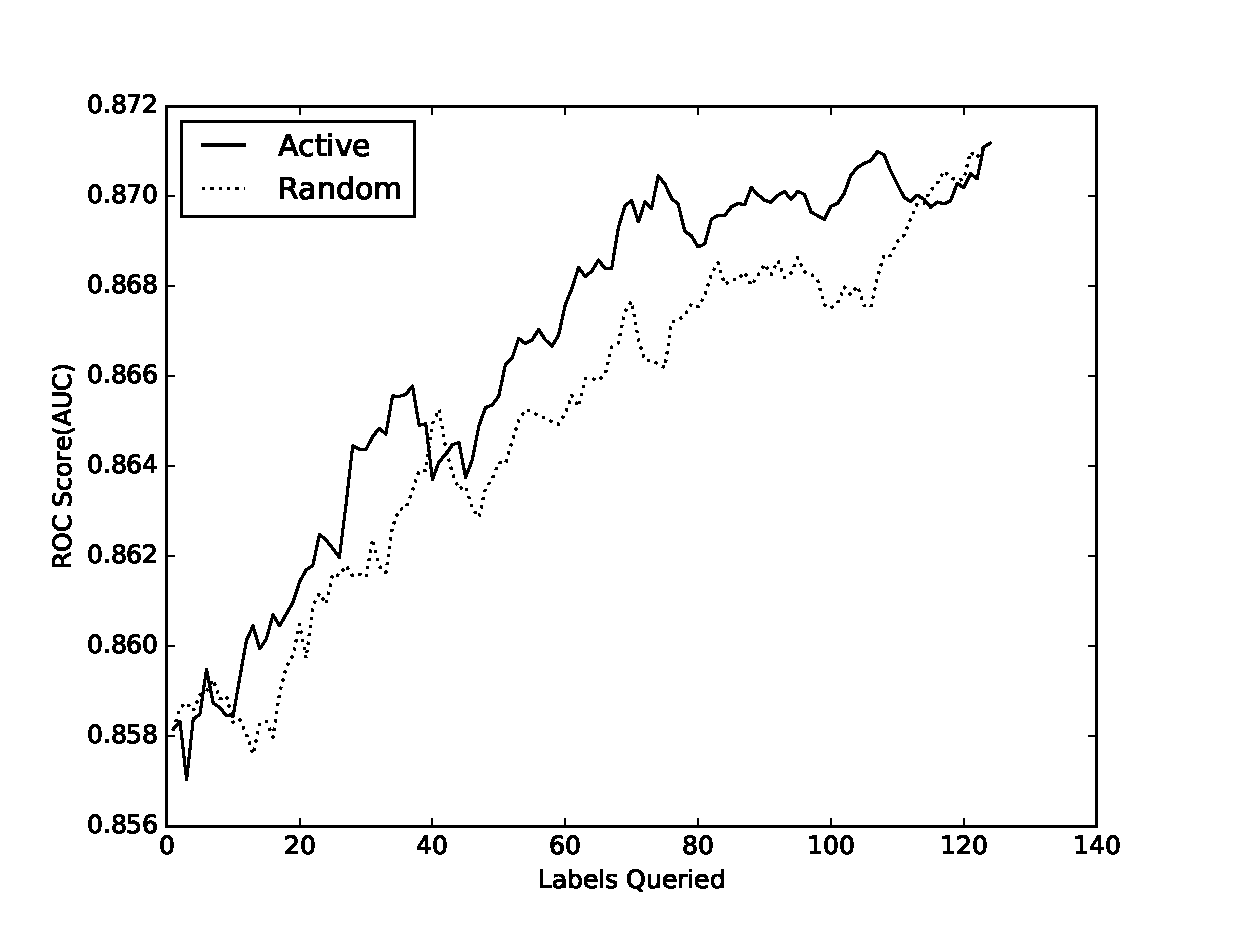
\includegraphics[scale=0.5]{plot}

The above plot shows the results of the evaluation for both the active learner and the baseline. The y-axis represents the ROC score and the x-axis is the query step. Though not by much, the active learner slightly out-paces the baseline. Of course both methods converge to the same ROC score of ~0.87. This is to be expected since after the final query step, both methods would have queried all the proteins in the training pool meaning both corresponding SVMs saw all training examples.

\section*{Conclusion}
As shown above, the active learning method shows slight improvement from the baseline. Higher improvment would have been desired, but potential reasons for the observed results may prove to be helpful in taking future directions.

The results observed may have been extensively affected by the way the evaluation was performed. The evaluation was unrealistic because all the proteins had the same number of training instances. In a real environment different proteins would have vastly different sizes and, as a result, different numbers of contained training instances. In the future, evaluation on batches that correctly corresponded to real proteins could be beneficial. 

The size of the query pool could have also affected the evaluation. In a real world scenario the active learner would have access to thousands of DNA-Protein complexes. With a more realistically sized query pool, the divergence between the ROC scores of the active learner and the baseline could possibly have been much larger. 

Another potential culprit is the assumption of linear separability. The noisiness of the labelled data invalidates this assumption and hence, the model cannot use a hard margin SVM. Because of this, the intution of the scoring method in \cite{active_learning} is somewhat lost. Further work would need to be done to the scoring function order to handle the loss of separability. As well switching to a method that does not consider version spaces might be beneficial as well.

\bibliographystyle{plain}
\bibliography{mybib}{}

\end{document}
